\chapter{Organisation du développement}
Introduction, pas eu de tâche particulière intégration au sein de l'équipe avec diff tâches (ajout fonctionnalités, correction bug, Documentation en aglais, refacto, optimisation, formation

\section{Gestion de projet agile}
\subsection{Méthodes agiles}
\paragraph{}
Le projet a été mené selon une approche agile. La gestion de projet agile repose sur un développement itératif qui consiste à découper un projet en plusieurs itérations appelé sprint. Les méthodes agiles définis plusieurs valeurs fondamentales : 
\begin{itemize}
\item La communication au sein de l'équipe
\item La collaboration avec le client, celui-ci doit être impliqué tous au long du développement.
\item L'adaptation au changement, c'est-à-dire que le planification initiale doit être flexible pour permettre l'évolution de la demande. 
\end{itemize}
Il existe différentes type de méthode agile (Scrum, XP, RAD...) qui possèdent leurs propres caractéristiques.
\paragraph{}
Pour le développement d'Open Orchestra, c'est la méthode Scrum qui est utilisé. Scrum définis trois rôles au sein d'une équipe : 
\begin{itemize}
\item  Le \og Product Owner (PO) \fg{} qui porte la vision du produit
\item Le \og Scrum Master \fg{} est le responsable de la mise en œuvre de la méthode, il doit s'assurer que cette dernière est correctement appliqué
\item L'équipe de développement qui est chargé de transformer les besoins exprimés par le Product Owner. 
\end{itemize}
\paragraph{}
La réalisation d'un projet utilisant la méthode est rythmée par différents évènements : 
\paragraph{}
Tous d'abord, le sprint qui est représente une période de courte durée, de une à quatre semaines, durant laquelle l'équipe effectue un nombre de tâches définis à l'avance.
 \paragraph{}
 La réunion de planification où l'équipe répond à deux questions, \og Quoi ? \fg{} c'est-à-dire les tâches du backlog\footnote{Le backlog est un ensemble de fonctionnalités ou de tâches nécessaire pour la réalisation satisfaisante d'un projet} qu'elle réalisera au prochain sprint et \og Comment ? \fg{} c'est a ce moment que l'équipe estime les tâches choisis au \og Quoi \fg{} 

 \paragraph{}
Le \og daily scrum \fg{} qui est une réunion réalisé quotidiennement. Durant cette réunion chaque membre de l'équipe indique les tâches qu'il a réalisé depuis le dernier daily et celles qu'il va effectuer jusqu'au prochaine daily et pour finir les difficultés qu'il a ou pense rencontrer.
Cette réunion permet à tous les membres de connaître les tâches de chacun afin de s'entraider et d'anticiper plus facilement les obstacles.
 \paragraph{}
Pour finir à la fin du sprint, les membres de l'équipe se réunisse pour la revue de sprint durant laquelle les différentes tâches réalisés durant le sprint sont présentés et validés. Puis pour la rétrospective qui permet de mettre en évidence les points positif et les actions a mettre en place pour améliorer le prochain sprint.

\begin{figure}[H]
  \begin{center}
    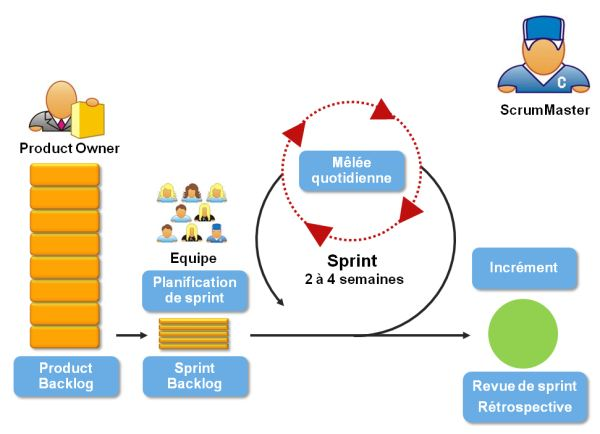
\includegraphics[scale=0.75]{images/scrum}
  \end{center}
  \caption{Schéma décrivant la méthode Scrum}
  \caption*{Source: http://www.agiliste.fr/fiches/guide-demarrage-scrum/}
  \label{scrum}
\end{figure}

\subsection{Scrum avec Open Orchestra}
Au sein du projet Open Orchestra, la méthode Scrum est appliqué.. Ainsi des sprint de une semaine avec un daily scrum tous les jours a midi.
De plus, tous les mercredis ou mardis selon les disponibilités une \og cérémonie \fg{} qui comprend la réunion de planification et la rétrospective.
Concernant, la revue de sprint (validation des taches du sprint) celle-ci n'est pas faite durant une réunion définis mais tout au long du sprint par le product ownver.
 \paragraph{}
 Pour faciliter la mise en place de la méthode Scrum, l'équipe utilise différent outils.
 Tous d'abord Skype et Slack\footnote{Slack est une plateforme de communication réalisé en 2014 qui permet d'intégrer facilement différents outils de service en ligne tel que github, trello, dropbox, google drive, ...)} pour la communication.
  \paragraph{}
 Et enfin Trello pour organiser les tâches, en effet l'équipe possédé un \verb?board? avec différentes colonnes pour organiser les tâches : 
 \begin{itemize}
 \item[]
 \item \textbf{Backlog} : le backlog qui contient les différentes tâches a effectué pour le projet, le tâches du backlog sont organisées en quatre colonnes (Nice to have, Good, Great, Must have) selon la priorité de la tâche.
 \item[]
 \item \textbf{Support} : Les demandes effectué par les différentes équipes d'intégrateur d'Open Orchestra au sein d'Interakting.
\item[]
 \item \textbf{Proposition} : Les différentes propositions d'amélioration ou de re- factorisation du code faites par les membres de l'équipe.
\item[]
 \item \textbf{Bugs} : Les différents bug rencontrés durant le développement
\item[]
 \item \textbf{Todo} : Les taches a effectuer durant le sprint en cours.
\item[]
 \item \textbf{Doing} : Les taches actuellement en développement.
\item[]
 \item \textbf{Blocked} : Les taches bloqué pour différentes raison (manque de précision de la tache, bug empêchant la réalisation de la taches)
\item[]
 \item \textbf{ToDeploy} : Taches réalisés qui sont prêtes a être déployé sur le serveur d'intégration.
\item[]
 \item \textbf{ToValidate} : Taches du sprint en attente de validation par le product owner.
\item[]
 \item \textbf{Failed} : Taches du sprint e non validé par le product owner
\item[]
 \item \textbf{Done} : Taches du sprint validé par le product owner
 \item[]
 \end{itemize}
Les colonnes \verb?ToDeploy?, \verb?Done? sont unique a un sprint, il y a donc une colonne  différent\verb?ToDeploy?, \verb?Done? pour chaque sprint.
\paragraph{}
Par exemple, une tâches suit un processus, présenté par le schéma, bien particulier entre l'intrégration de la tache dans la sprint et ca validation par le product ownver. Ce processus permet de suivre facilement l'avancement ou encore les différents problèmes rencontrés sur les différentes tâches par tous les membres de l'équipe.
\section{Intégration continue}
Pour le développement d'Open Orchestra les principes de l'intégration continue sont utilisés. 
\newline
\begin{quotation}
L'intégration continue est un ensemble de pratiques utilisées en génie logiciel consistant à vérifier à chaque modification de code source que le résultat des modifications ne produit pas de régression dans l'application développée.
\end{quotation}
\textit{Source wikipedia}

L'utilisation de ces pratiques apporte de nombreux avantages, tous d'abord comme il est indiqué dans la citation cela permet de minimiser les régréssions mais aussi d'avoir a tous moment un produit (logiciel, site, etc) utilisable.
\paragraph{}
La mise en place de cette technique nécessite différentes pré-requis : 
\begin{itemize}
\item[]
\item Dépôt unique de code source versionné
\item Automatisation des tests
\item Un environnement similaire a celui de production
\item Automatiser le déploiement
\end{itemize}

\subsection{Git}
Dans le cadre d'Open Orchestra, le code source est versionné avec git\footnote{Git est un logiciel de versionning décentralisé, c'est-à-dire qu'il n'existe pas un dépôt unique mais un dépôt local pour chaque développeurs.} et utilise GitHub qui est un service web permettant d'héberger un dépôt git. Comme je l'expliquais lors des présentations des caractéristiques d'Open Orchestra, ce dernier est découpé en plusieurs bundles et donc chaque bundles possède son propre dépôt sur GitHub.
\paragraph{}
Open orchestra étant toujours en version bêta, il n'y a pas de realease a proprement parlé. Ainsi le worklow de développement sur github est simplifié car il n'y a qu'une seule branche stable, la branche master. Les autres branches sont des branches temporaires d'ajout de fonctionnalités ou de correction de bugs. Ce type de workflow est appelé \verb?GitHub flow? et est représenté par le schéma~\ref{github}.
\begin{figure}[H]
  \begin{center}
    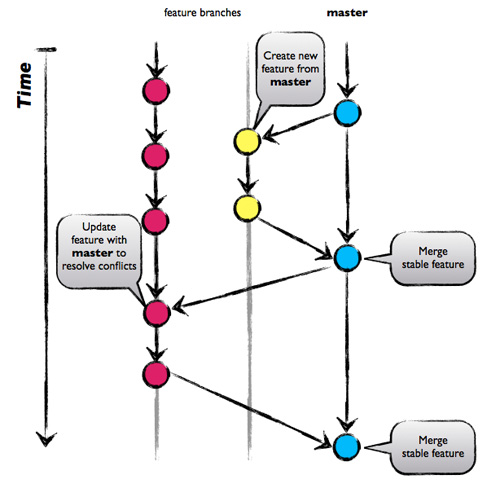
\includegraphics[scale=0.75]{images/github-flow}
  \end{center}
  \caption{Exemple d'architecture d'utilisation d'Open Orchestra}
  \caption*{Source: http://nicoespeon.com/fr/2013/08/quel-git-workflow-pour-mon-projet}
  \label{github}
\end{figure}

\paragraph{}
Ainsi avec ce type de workflow, la modification du code source que ce soit pour corriger un bug ou ajouter une fonctionnalités s'effectue toujours de la même manière : 
\begin{enumerate}
\item[]
\item Mettre à jour sa branche master en local
\item Créer une nouvelle branche en local à partir de master
\item Effectuer les modifications dans cette branche
\item Pousser sa branche sur GitHub (origin)
\item Vérifier que les tests fonctionnne, je reviendrais plus en détail sur ce point par la suite
\item Ouvrir une pull-request, sur GitHub une pull-request consiste à faire une proposition de modification, à partir de cette pull-request les différents membres peuvent commenter, valider ou non la modification.
\end{enumerate}

Une fois la pull-request validé, elle peut être mergé avec master, c'est-à-dire inclure la modification dans la branche master.
\paragraph{}
Comme je l'ai précisé en début de section pour le moment Open Orchestra ne possédé pas de branche realease. Toutefois le projet Open Orchestra est déjà utilisé par des intégrateurs pour réaliser des sites a distanciation de différent clients, il ne peuvent donc pas utiliser directement la branche master, ils leurs fait des points d'arrêts. Pour cela, sauf cas particulier (bug bloquant, besoins particulier) la branche master est \verb?taggé? toute les deux semaines environs ainsi cela permet à l'équipe d'Open Orchestra de continuer le développement  du projet et aux intégrateurs d'avoir un version fixe de la branche master qu'il mettre à jour au moment le plus opportunt pour eux.  Lorsque Open Orchestra ne sera plus en bêta cela changera la version 1 aura sa propre branche dans la quelle aucune nouveautés sera intégré or mis les corrections de bug.

\subsection{Travis CI}
Lorsqu'une branche est poussé sur l'un des dépôts GitHub du projet, les tests sont automatiquement lancé. Pour cela, les différents dépôts du projet intégre un outil \verb?Travis CI?. Travais CI est un service qui est liée a GitHub, il permet de lancer à déclencher un certains nombre de tâches lors d'événement sur le dépôt. Dans le cas d'Open Orchestra Travis CI permet de lancer les tests unitaires après chaque \verb?push? sur un dépôt. Un des avantages de travis est qu'il se configure très facilement grâce un fichier yaml.
\paragraph{}
Par exemple le fichier de configuration travis d'un des dépôts d'Open Orchestra 
\begin{verbatim}
    language: php

    php:
          - 5.4

    install:
          - composer install --prefer-dist --no-progress
 
    script: ./bin/phpunit
\end{verbatim}

Indique que le langage utilisé est php et que les tests doivent être exécuté avec la version 5.4 de php et enfin avant d'exécuter \verb?phpunit? pour lancer les test il est demandé a travis de faire un \verb?composer install? pour récupérer les dépendances du projet.  Ensuite à partir de ce fichier de configuration Travis CI est capable de créer l'environnement pour effectuer les tests, il est bien sûr possible d'aller plus loin dans  personnalisation de l'environnement en allant cherchant d'autre dépendances avec \verb?apt-get install? par exemple ou encore de demander a être notifié par email si les tests ne passe pas.

\subsection{Déploiement}
Le déploiement sur un serveur de production n'est pas toujours une tâche facile(uploader le code, mettre à jour les dépendances, lancer les migrations de la base de données, vider le cache, etc)  or pour permettre une intégration continue il est nécessaire de déployer régulièrement son application, il semble donc nécessaire d'automatiser cette taches pour cela il existe de nombreux outils. 
\paragraph{}
En ce qui concerne Open Orchestra nous utilisons \verb?Capistrano?. \verb?Capistrano? est un outil écrit en Ruby qui permet d'exécuter des scripts sur un ou plusieurs serveur. Il est principalement utilisé pour faire du déploiement mais il permet aussi de créer ces propres par exemple pour Open Orchestra nous l'utilisons aussi pour lancer des tests de charge, avec Jmeter, directement sur le serveur d'intégration.
\paragraph{}
Un autre avantage \verb?Capistrano? est qu'il permet de revenir facilement sur une version précédente de votre application grâce a une architecture de dossier que met en place \verb?Capistrano? dans le dossier de votre application sur serveur : 
\begin{verbatim}
/app/
       releases/ Contient un dossier pour chaque déploiement estampillé
       current lien symbolique pointant vers un dossier de release spécifique
       shared/ Contient les données partagées entre chaque déploiement
\end{verbatim}
Ainsi, si un déploiement provoque des erreurs, il suffit de faire pointé le lient symbolique \verb?current? vers une autre version.

\section{Qualité}
L'équipe d'Open Orchestra essaye de fournir un produit de qualité que ce soit au niveau du code, du couplage ou encore du fonctionnel. Pour cela différente pratique, outils sont mise en place.
\subsection{Qualité du code}
Tous d'abord au niveau du code Open Orchestra utilise le standard PSR-2. PSR-2 est un ensemble de recommandation sur le style et l'organisation du code dont voici les plus importantes : 
\begin{itemize}
\item[]
\item La tag de fermeture \verb?\?>. doit être omis de tous les fichiers contenant uniquement du PHP
\item Tous les fichiers PHP doivent se terminer par une ligne vide.
\item La visibilité doit être déclarée sur toutes les propriétés et méthodes.
\item L'ouverture des accolades pour les classes, les méthodes doit figurer sur la ligne suivante, les accolades de fermeture DOIVENT figurer sur la ligne suivante après le corps de la classe.
\item Il doit y avoir un espace après la structure clé de contrôle et pas d'espace après la parenthèse ouvrante et avant la parenthèse fermante
\item Il doit y avoir un espace entre la parenthèse fermante d'une structure de contrôle et de l'accolade
 ouvrante
 \item L'accolade fermante d'une structure de contrôle doit être sur la ligne suivante après le corps
 \item[]
\end{itemize}
\paragraph{}
Utiliser cette recommandations permet une harmonisation du code et ainsi il est plus simple pour toute l'équipe de relire et reprendre le code d'un autre membre mais aussi pour tous les développeurs qui utilise Symfony 2 puisque ce dernier utilise aussi les recommandations PSR-2
\paragraph{}
Lors de revue de code des pull-request, il n'est pas toujours aisé de détecter l'utilisation des bonnes pratiques ou non. Il existe des outils qui permettent d'analyser le code automatiquement et de détecter les oublis lors de la revue.
\paragraph{}
Pour le projet Open Orchestra deux outils sont utilisés : 
\paragraph{}
Tous d'abord, Code Climate s'interface avec les dépôts c'est à dire que lors d'un push le code est analysé.
Code Climate permet de détecter la duplication de code, la couverture des tests, la qualité globale du projet. De plus, il fournis une note indique la qualité globale du dépôt. 
Le second outil est SensioInsignt fonctionne de la même façon que Code Climate mais en supplément des vérifications sur les bonne pratiques de Symfony 2.
\subsection{Test}
Le plus grand intérêt des tests est qu'ils permettent de réduire les régressions lorsque l'on applique des modifications a une applications. En effet, lorsqu'une application devient assez conséquente il n'est pas toujours aisé d'anticiper toutes les répercutions lorsque l'on modifie une portion de code. Les tests permettent donc de tester l'ensemble de l'application et ainsi vérifier que cette dernière fonctionne toujours correctement après les modifications effectué. 
De plus, ils sont en générale gage de qualité
 \paragraph{}
 Il existe deux grandes familles de test, Tous d'abord les tests unitaires qui permettent de vérifier que chaque méthode et fonction fonctionne correctement, les test doit être indépendant au maximum les uns des autres pour cela il existe les mocks qui sont des objets qui permettent de simuler le comportement d'objets \og{}réels\fg{}.
 D'autre part les tests fonctionnels qui eux contrairement aux tests unitaires les fonctionnalités de bout en bout. c'est-à-dire qu'ils toutes les couches de l'application (routing, modèle, action, controlleurs, template).
  \paragraph{}
 Avec Symfony, il est assez facile de créer des tests puisqu'il intègre la bibliothèque PHPUnit qui fournis un framework de test complet, de plus pour les tests fonctionnels Symfony propose une class WebTestCase qui permet d'initier le noyau de Symfont, elle fournis notamment un objet \verb?client? qui permet d'effectuer des requêtes HTTP sur son application et un crawler qui permet de vérifier si le résultat de la requêtes est correct .
  \paragraph{}
 Avec ces deux types de tests toutes les fonctionnalités d'une application ne sont pas encore couverte, il reste encore l'IHM (Interface Homme Machine) qui est a mon avis une des parties les plus dur a tester puisqu'elle peut intégrer notamment du JavaScript, ce qui rend les tests côté serveur que nous avons vue précédemment inutile. 
 
Test unitraite, Test fonctionel, (Mise en place de test  pour tous les codes metiers) 
Behat (mise en place de test behat) 
\subsection{Qualité fonctionnel}
Fonctionnel
